\section{Применение локальных оценок константы Гёльдера для ускорения сходимости}
Как видно из описания метода, независимо от локальных свойств оптимизируемой одномерной
функции, для вычисления характеристик всех интервалов используется одно и то же
значение оценки константы Гёльдера. В работах [] было предложено использовать различные
значения M для каждого интревала, а также показана эффективность такого подхода в
случае одномерной оптимизации функций, удовлетворяющих условию Липшица. В работе []
рассмотрено применение адаптивных оценок констант Липшица в схеме многомерной вложенной оптимизации.

Для каждого интревала локальная оценка константы является аддитивной свёрткой
<<глобальной>> и <<локальной>> компонент (\(\gamma\) и \(\lambda\) соответственно):
\begin{displaymath}
  \begin{array}{lr}
    \lambda_i=\max\{H_{i-1},H_i,H_{i+1}\} \\
    H_i=\frac{|z_i-z_{i-1}|}{\Delta_i} \\
    H^k=\max\{H_i:i=2,\dots ,k\} \\
    \gamma_i=H^k\frac{\Delta_i}{\Delta^{max}} \\
    \Delta^{max}=\max\{\Delta_{i}:i=2,\dots ,k\}
  \end{array}
\end{displaymath}
\begin{equation}
\label{additiveConv}
M_i=r\cdot \max\{H_i, \frac{1}{2}(\lambda_i+\gamma_i),\xi\}
\end{equation}

Данный вариант свёртки не зависит от параметра \(r\), однако в [] также рассматривается
и адаптивная свёртка:
\begin{equation}
\label{additiveAdaptiveConv}
M_i=r\cdot \max\{H_i, \frac{\lambda_i}{r}+\frac{r-1}{r}\gamma_i,\xi\}
\end{equation}

Если априори известно, что оптимизируемая функция имеет сложный рельеф с множеством
локальных минимумов, то \(r\) изначально задаётся большим, что ведёт к преобладанию в
адаптивной свёртке «глобальной» сооставляющей \(\gamma\).

В [] приведена теорема о сходимости метода в случае, если целевая функция липшицева,
однако, как правило, подобные утверждения справедливы и в Гёльдеровой метрике, поэтому,
предположительно, будет верна следующая теорема:
\begin{hypothesis}
Assume the objective function \(f(x)\) to  satisfy Hölder condition with finite
constant \(H > 0\), and let x be a limit point of \(\{x_k\}\) generated by the algorithm.
Then, the following assertions hold:
\begin{enumerate}
  \item If \(x\in(0;1)\), then convergence to \(x\) is a bilateral one i.e. there
  exists two infinite subsequences of \(\{x_k\}\) converging to \(x\): one from the
  left, the other from the right;
  \item \(f(x_k) \geqslant f(x)\) for all trial points \(x_k, k \geqslant 1\);
  \item If there exists another limit point \(x^* = x\), then \(f(x) = f(x^*)\);
  \item If the function \(f(x)\) has a finite number of local minima in \([0, 1]\),
  then the point \(x\) is a local optimum;
  \item (Sufficient conditions for convergence to a global minimizer). Let \(x^*\)
  be a global minimizer of \(f(x)\). If there exists an iteration number \(k^*\)
  such that for all \(k > k^*\) the inequality
  \(M_j(k) > H_j(k)\) holds, where \(H_j(k)\) is the Hölder constant for the interval
  \([x_{j(k)-1}, x_{j(k)}]\) containing \(x^*\), and \(M_{j(k)}\) is its estimate.
  Then, the set of limit points for the sequence \(\{x_k\}\) coincides with the set
  of global minimizers for the function \(f(x)\).
\end{enumerate}
\end{hypothesis}

Доказательство теоремы требует отдельных теоретических исследований. В рамках данной
работы оно не будет проведено, наличие сходимости установлено только численно.

Эксперименты по оценке эффективности метода с локально-адаптивной оценкой константы
Гёльдера производились на двумерных классах задач Гришагина (Fgr) [] и GKLS Simple 2d [].
Каждый из классов содержит 100 многоэкстремальных функций. Развёртка во всех экспериментах
строилась с плотностью \(m=12\), параметр \(\varepsilon\) в критерии остановки был равен \(10^{-3}\).
Параметр \(r\) выбирался минимально возможным, при котором заданный метод решает все
задачи класса. Шаг поиска \(r\) равен 0,1.

\begin{figure}[ht]
    \centering
    \subfloat[global \(H\) estimation]{{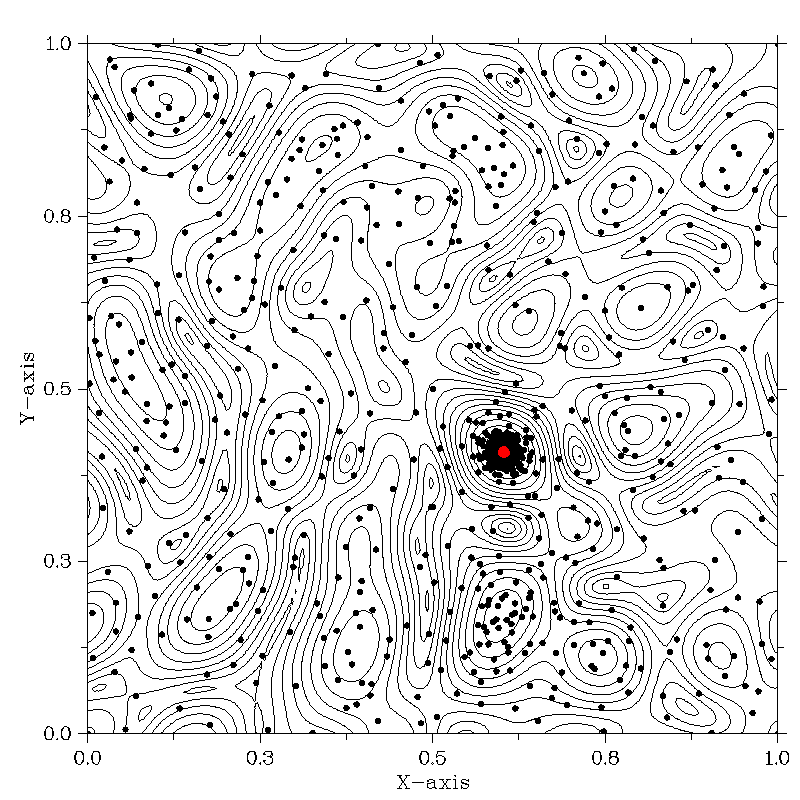
\includegraphics[width=0.45\textwidth]{images/gs_glob.png} }}
    \qquad
    \subfloat[local-adaptive \(H\) estimation]{{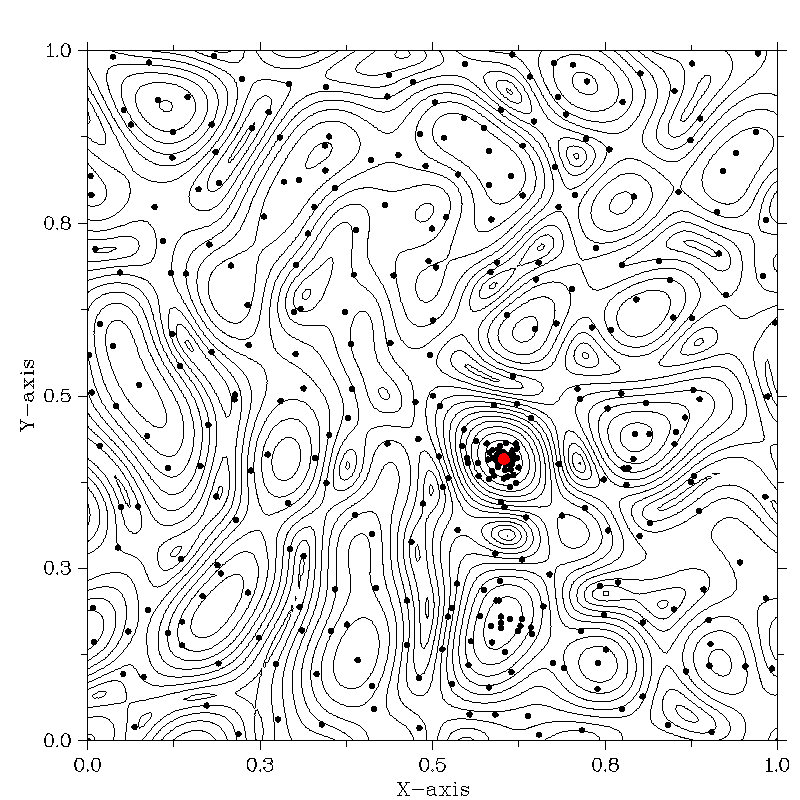
\includegraphics[width=0.45\textwidth]{images/gs_loc.png} }}
    \caption{The level lines of a function from \(F_{GR}\) class}
    \label{fig:grish_isolines}
\end{figure}

Для наглядной иллюстрации преимущества локально-адаптивной схемы оценки константы
\(H\) рассмотрим результаты работы метода на конкретном примере. На рис. [] показаны
линии уровня одной из функций класса Fgr и точки испытаний, проведённых методом с глобальной
оценкой константы Гёльдера и с оценкой по формуле (). Как видно из рисунков, метод с
глобальной оценкой константы проводит большое число испытаний в окрестности точки
глобального минимума прежде (всего проведено 1086 испытаний), чем выполнится условие
остановки, в то врямя, как метод с локально-адаптивной оценкой гораздо быстрее
сходится (всего проведено 385 испытаний). Аналогичная ситуация имеет место при
оптимизации одной из функций класса GKLS Simple 2d (рис. []). Метод с глобальной
оценкой константы произвёл 2600 испытаний, а метод с локально-адаптивной оценкой – 1190.

\begin{figure}[ht]
    \centering
    \subfloat[global \(H\) estimation]{{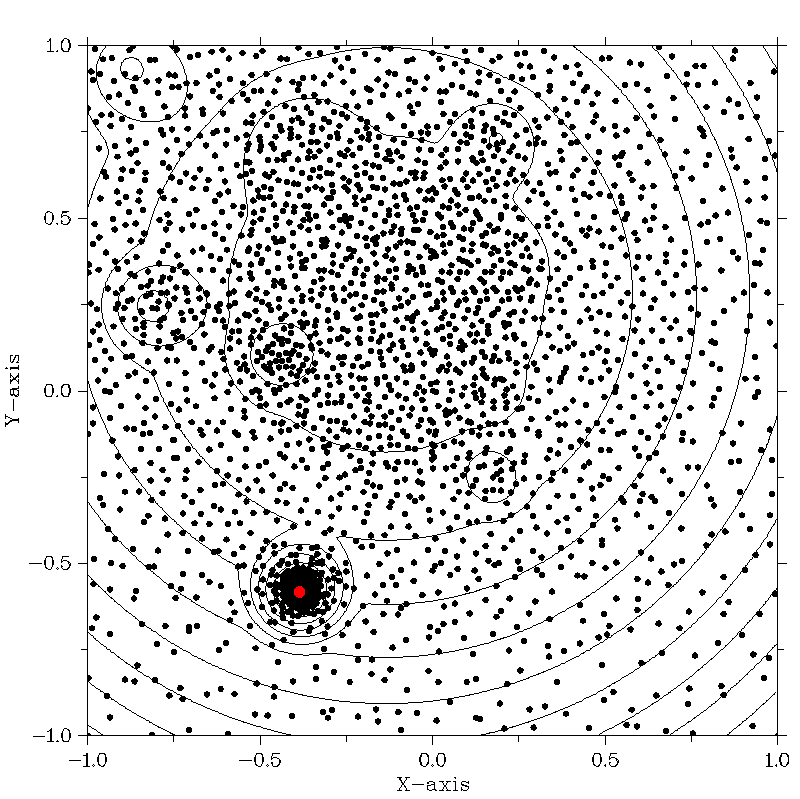
\includegraphics[width=0.45\textwidth]{images/gkls_glob.png} }}
    \qquad
    \subfloat[local-adaptive \(H\) estimation]{{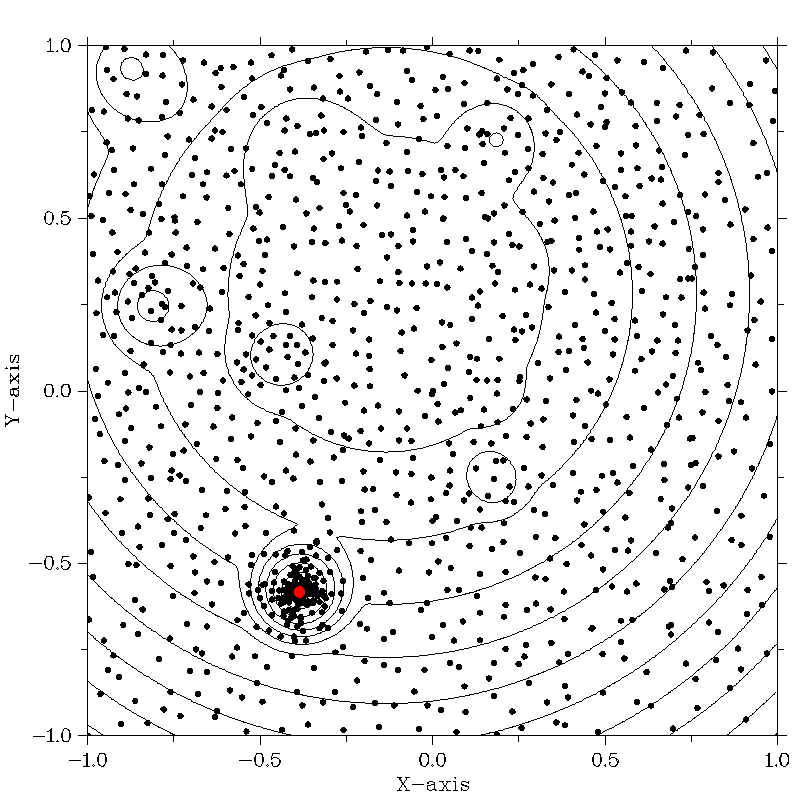
\includegraphics[width=0.45\textwidth]{images/gkls_loc.png} }}
    \caption{The level lines of a function from GKLS class}
    \label{fig:gkls_isolines}
\end{figure}

Далее перейдём к сравнению различных вариантов метода на рассматриваемых классах задач.
В качестве оценки эффективности алгоритма будем использовать, операционную характеристику,
описанную в [].

Как видно из операционных характеристик на рис. [], оба метода с локально-адаптивной
оценкой константы Гёльдера показали существенное преимущество, однако они требуют
задавать более высокое значение параметра \(r\). Если сравнивать между собой методы с
адаптивной и неадаптивной свёрткой [], то наглядно видно преимущество последнего,
хотя он и требует большее значение параметра надёжности \(r\) для решения задач из класса GKLS.

\begin{figure}[ht]
  	\center
    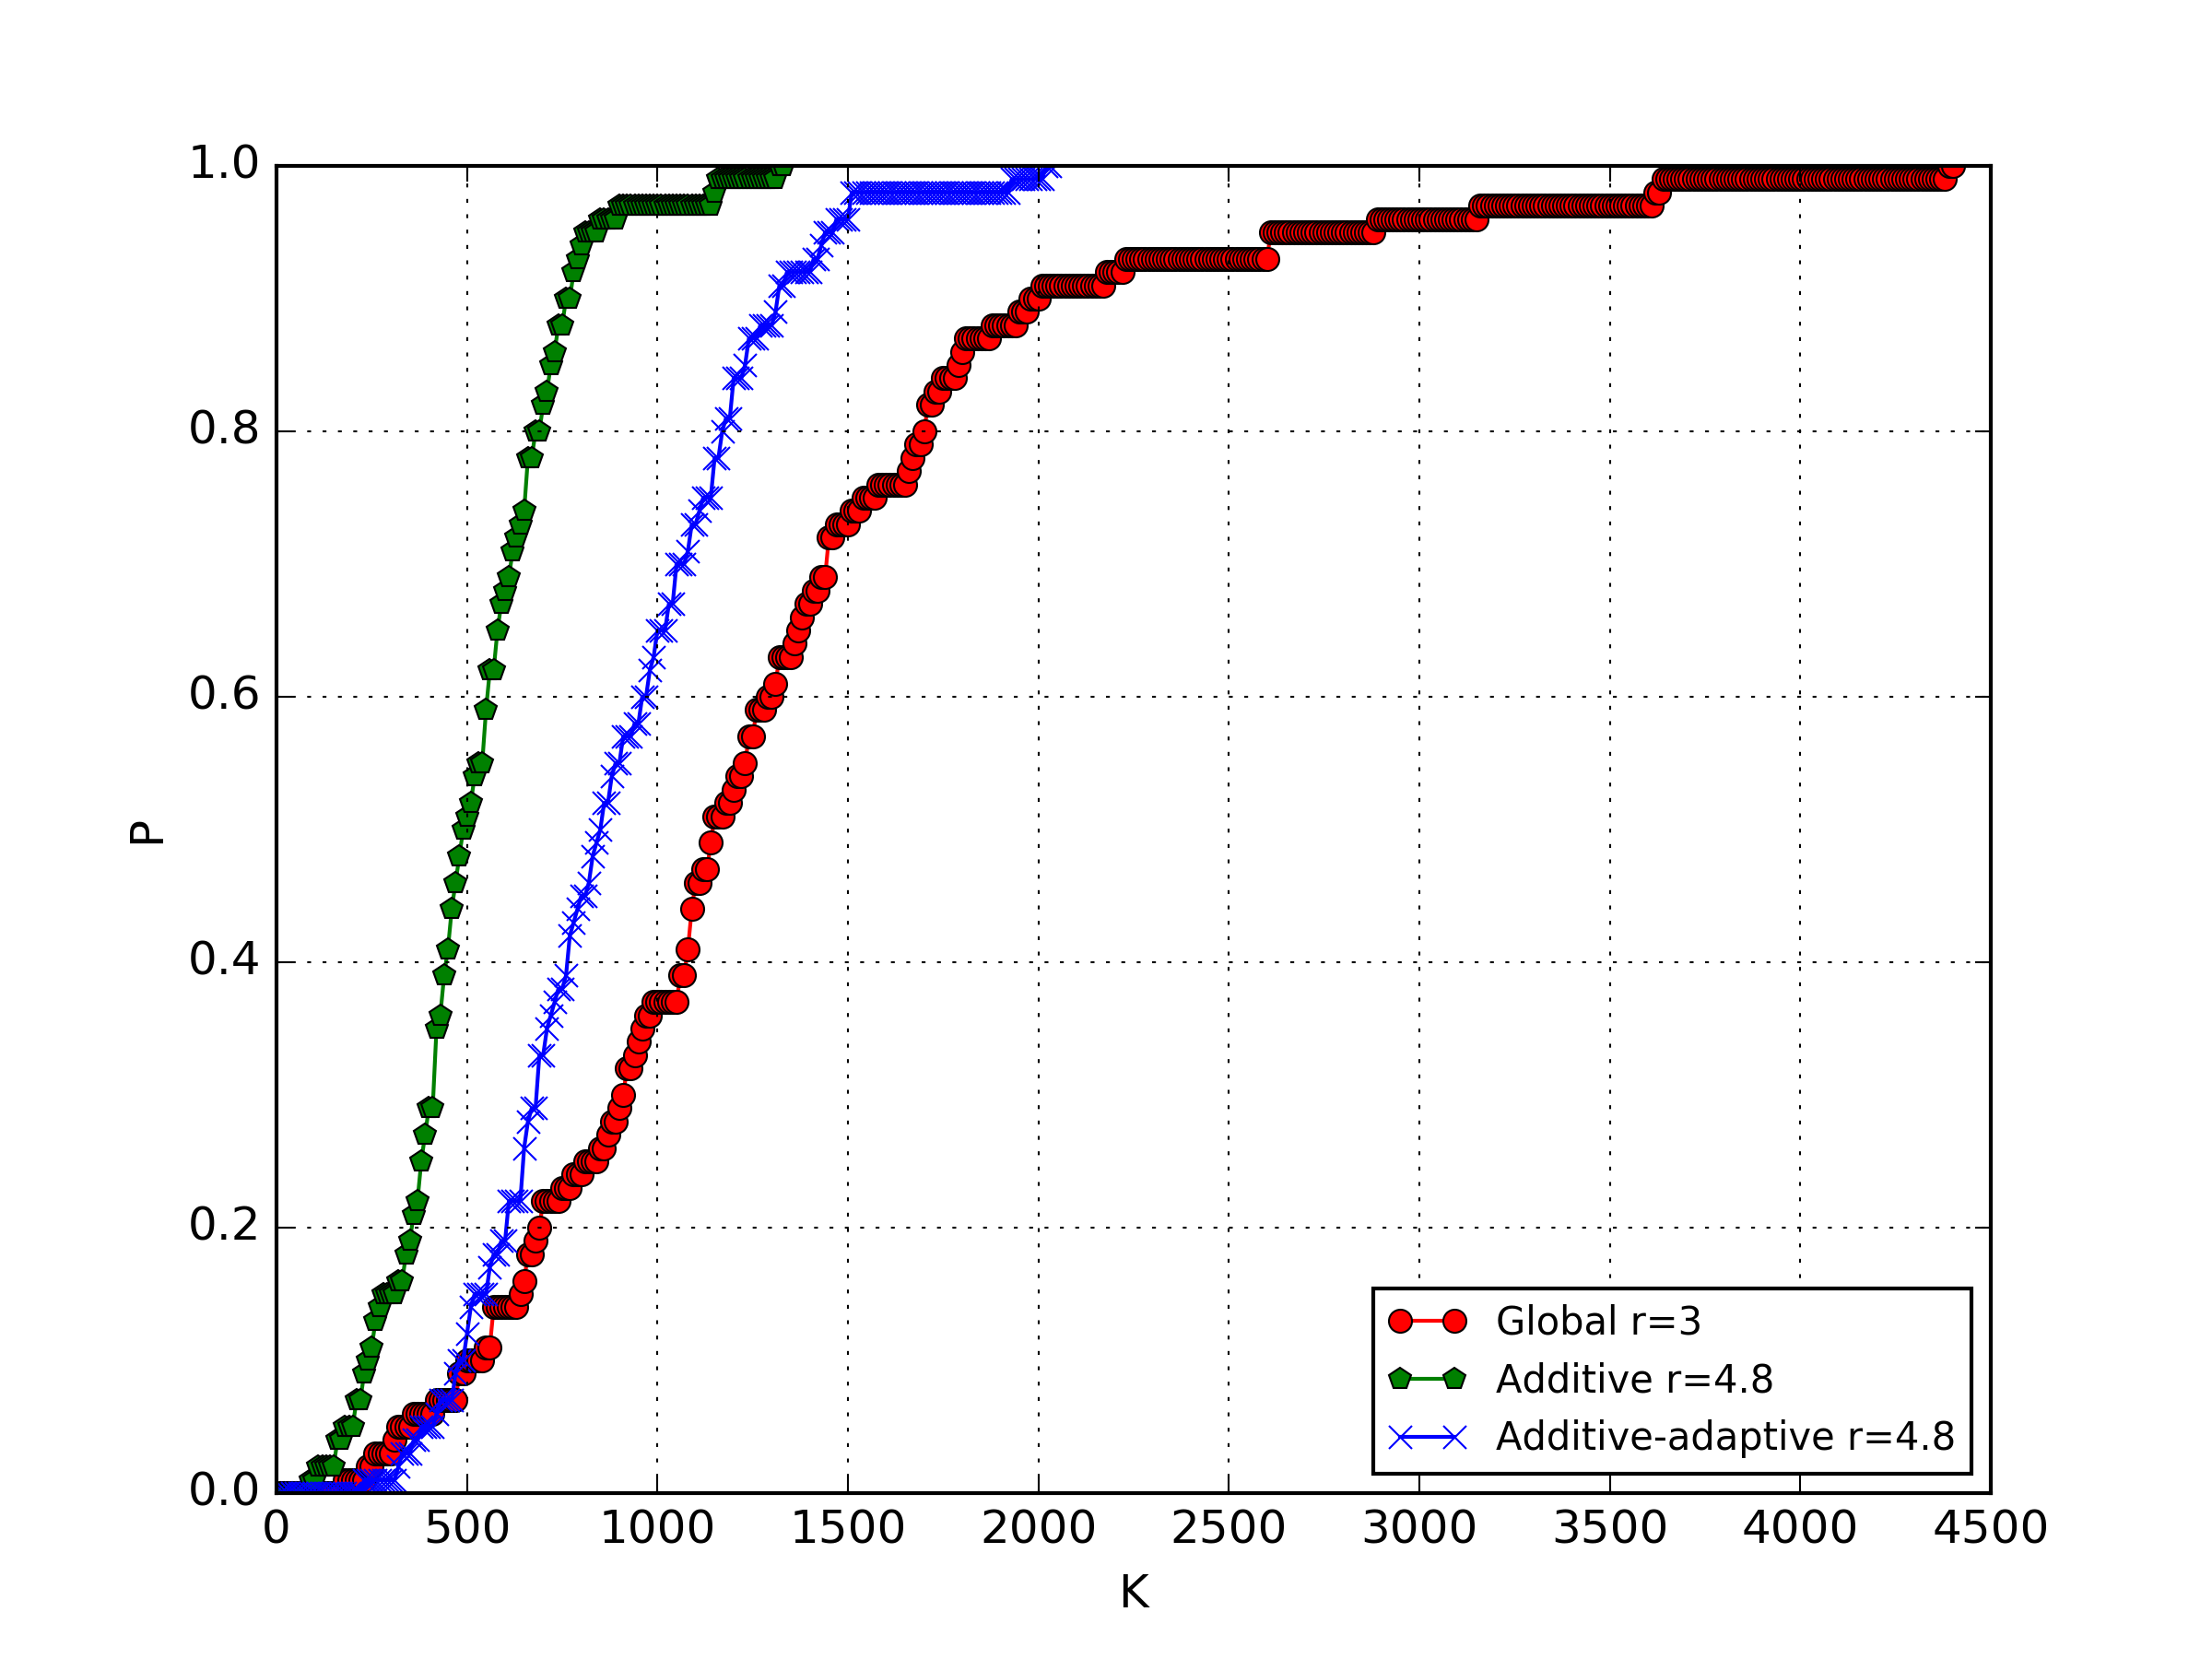
\includegraphics[width=0.75\textwidth]{images/grishagin.png}
    \caption{Operating characteristics of the methods compared on \(F_{GR}\) problems class}
    \label{fig:grishh_op}
\end{figure}

\begin{figure}[ht]
  \center
  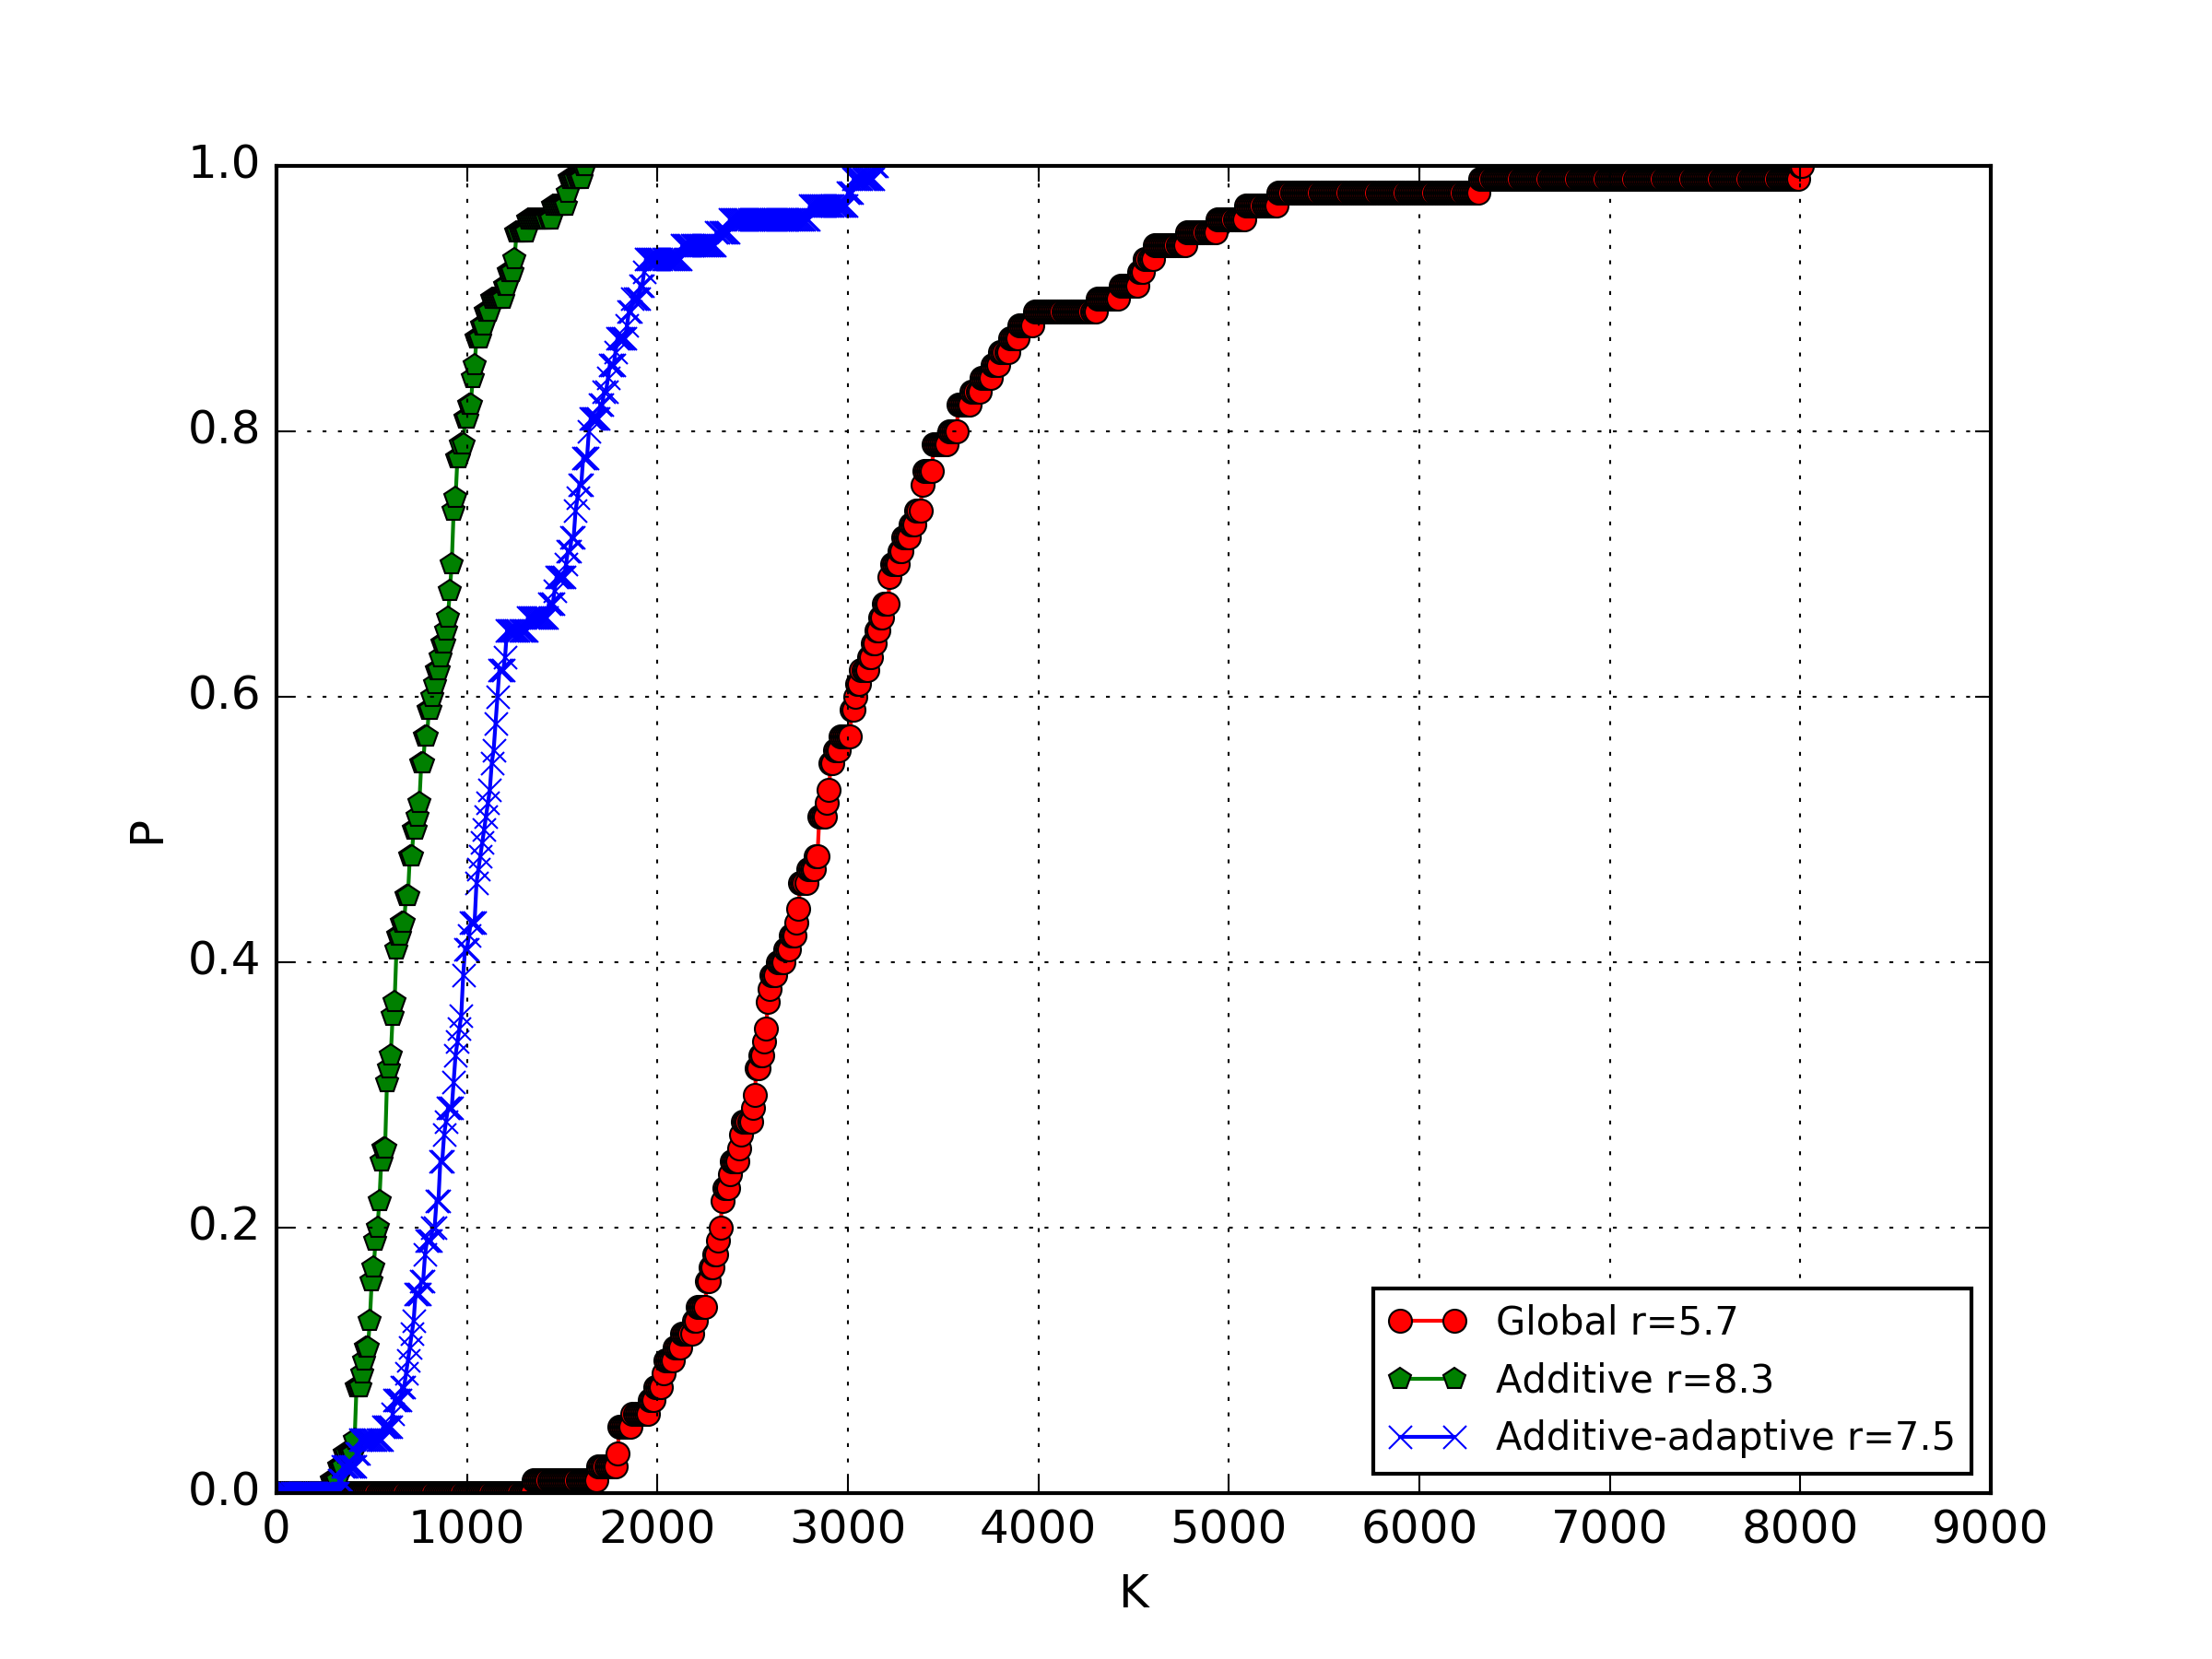
\includegraphics[width=0.75\textwidth]{images/gkls-s.png}
  \caption{Operating characteristics of the methods compared on GKLS problems class}
  \label{fig:gkls_op}
\end{figure}
